\documentclass{beamer}
\usepackage{etoolbox}
\newtoggle{german}

% % % % % LANGUAGE % % % %
% Make your choice here
\togglefalse{german} % English
%\toggletrue{german} % German
% % % % % \LANGUAGE % % % %

\iftoggle{german}{
\usepackage[ngerman]{babel} % Deutsche Sprachanpassungen
\usepackage[T1]{fontenc}    % Silbentrennung bei Sonderzeichen
\usepackage[utf8]{inputenc} % Direkte Angabe von Umlauten im Dokument.Wenn Sie an einem Mac sitzen,verwenden Sie ggf. „macce“ anstatt „utf8“.
\usepackage[autostyle=true,german=quotes]{csquotes} % Anfuehrungszeichen\
}{
\usepackage[utf8]{inputenc}}

\usepackage{makecell}
\usepackage[utf8]{inputenc}
\usepackage[T1]{fontenc}
\usepackage{textcomp}
\setbeamercovered{transparent}
\usepackage{default}
\usepackage{lmodern}
\usepackage{amsmath,amsfonts,amssymb} % Mathe
\usepackage{eurosym}
\usepackage{tikz}
\usepackage{graphicx}
\usepackage[labelformat=empty]{caption}
\usepackage{verbatim}
\usepackage{color}
\usepackage{hypernat}
\usepackage{tabularx}
\usepackage[]{units}
\usepackage{caption}
\usepackage{comment}
\usepackage{subfigure}
\usepackage{wasysym}
\usepackage{ulem}
\usepackage[printonlyused]{acronym} 
\usepackage{tabularx}
\usepackage{appendixnumberbeamer}
\usepackage{epigraph}
\usepackage{remreset}% tiny package containing just the \@removefromreset command
\usepackage{./pdfpcnotes}% Usefull package for notes for presentations

\setbeamercolor{background canvas}{bg=}%transparent canvas
%\usepackage{draftwatermark}
%\SetWatermarkLightness{0.8}
%\SetWatermarkScale{0.75}
%\SetWatermarkColor[gray]{0.9}

\let\Tiny=\tiny % Reduces a few recent error on Unix systems

\usepackage[sorting=none,style=numeric-comp,backend=bibtex,firstinits=true]{biblatex} % load the package
\addbibresource{./references.bib} % Add your bib file
\renewcommand*{\bibfont}{\footnotesize}

% % % % Style % % % %
% Some colours as used in other programms like openoffice
\definecolor{red}{RGB}{184,71,71}
\definecolor{green}{RGB}{51,204,102}
\definecolor{blue}{RGB}{0,153,255}
\definecolor{fhblau}{rgb}{0, 0.594, 0.949}

\setbeamercolor{title}{bg=fhblau, fg=white}
\setbeamercolor{frametitle}{bg=fhblau, fg=white}
\setbeamercolor{structure}{fg=fhblau}

% MISC Styles %
\setbeamertemplate{bibliography item}[text]
\usetheme{default}
\setbeamertemplate{footline}[frame number]
\setbeamersize{text margin left=0.3cm,text margin right=0.3cm}
\setbeamertemplate{navigation symbols}{}%remove navigation symbols
\makeatletter
\@removefromreset{subsection}{section}
\makeatother
\setcounter{subsection}{1}


% Here are some usefulf different fonts. Use them in every flooting enviroment with \usebeamerfont{AAA}
\setbeamerfont{AAA}{size*={16.00}{15.00}}
\setbeamerfont{aaa}{size*={12.00}{11.00}}
\setbeamerfont{bbb}{size*={11.00}{11.00}}
\setbeamerfont{ccc}{size*={10.00}{11.00}}
\setbeamerfont{ddd}{size*={9.00}{11.00}}
\setbeamerfont{eee}{size*={8.00}{11.00}}
\setbeamerfont{fff}{size*={7.75}{10.75}}
\setbeamerfont{ggg}{size*={7.50}{10.50}}
\setbeamerfont{hhh}{size*={7.25}{10.25}}
\setbeamerfont{iii}{size*={7.00}{10.00}}
\setbeamerfont{jjj}{size*={6.00}{9.00}}
\setbeamerfont{kkk}{size*={5.00}{8.00}}
\setbeamerfont{lll}{size*={4.00}{7.00}}
\setbeamerfont{mmm}{size*={3.00}{6.00}}
\setbeamerfont{nnn}{size*={2.00}{5.00}} 

% Set some beamer fonts
\setbeamerfont{title}{size=\Large,series=\bfseries,parent=structure}
\setbeamerfont{caption}{size=\footnotesize \itshape}
\setbeamertemplate{footline}[text line]{%
	\parbox{\linewidth}{\vspace*{-8pt}\hspace{1em}\insertshortauthor\hfill\insertpagenumber}}

\renewcommand*{\bibfont}{\usebeamerfont{kkk}}

% A new cell type
\newcommand{\specialcell}[2][c]{%
  \begin{tabular}[#1]{@{}c@{}}#2\end{tabular}}

% This is usefull if you want to use enumerations over several frames
\newcounter{saveenumi}
\newcommand{\seti}{\setcounter{saveenumi}{\value{enumi}}}
\newcommand{\conti}{\setcounter{enumi}{\value{saveenumi}}}

% logo of my university
\titlegraphic{
\centering %
\includegraphics[height=1.5cm]{./logos/logo_hbrs.png} \hspace{2cm} % For external companies

\includegraphics[height=1.5cm]{./logos/logo_hbrs.png}}


% % % % % Opening % % % %
\title[]{Semantic Segmentation using Resource Efficient Deep Learning}

\author[Naresh Kumar Gurulingan|]{Naresh Kumar Gurulingan \\ \footnotesize naresh.gurulingan@smail.inf.h-brs.de}
\date{\today}
\institute[HBRS]{Hochschule Bonn-Rhein-Sieg}


\begin{document}

% Title Frame
\begin{frame}
\pnote{Here are some notes. They are not visible on the first slides} % Notes
\titlepage
\end{frame}

\iftoggle{german}{
\begin{frame}{Agenda}
\usebeamerfont{ccc}
\tableofcontents
\end{frame}
}{
\begin{frame}{Table of Contents}
\usebeamerfont{ccc}
\tableofcontents
\end{frame}
}

% First Frame
\begin{frame}
	\frametitle{Overview of the dataset}
	\section{Overview of the dataset}
		\textbf{Objects in the dataset:}
		\begin{figure}
			\centering
			\captionsetup[sub]{font=small,labelfont={bf,sf}}
			\subfigure[axis]{\label{fig:a}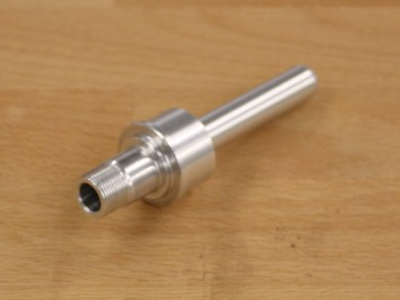
\includegraphics[width=17mm]{images/axis}}
			\hfill{}
			\subfigure[bearing]{\label{fig:b}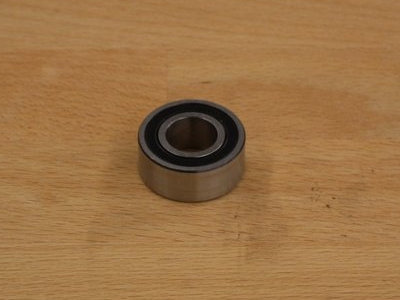
\includegraphics[width=17mm]{images/bearing}}
			\hfill{}
			\subfigure[bearing box AX01]{\label{fig:c}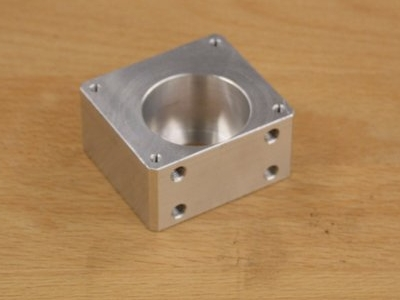
\includegraphics[width=17mm]{images/bearingBoxAX01}}
			\hfill{}
			\subfigure[bearing box AX16]{\label{fig:d}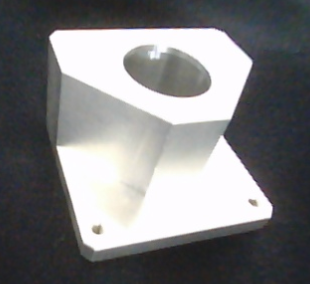
\includegraphics[width=16mm]{images/bearingBoxAX16}}
			\hfill{}
			\subfigure[container blue]{\label{fig:e}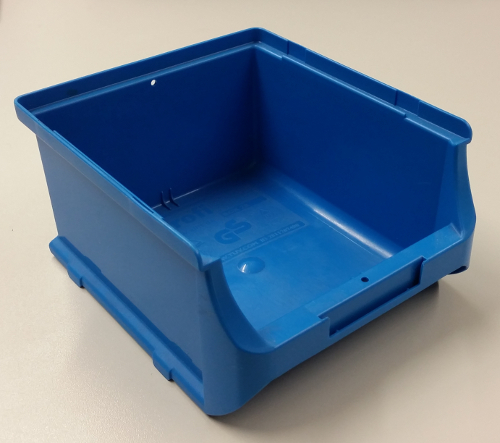
\includegraphics[width=16mm]{images/container_blue}}
			\hfill{}
			\subfigure[container red]{\label{fig:f}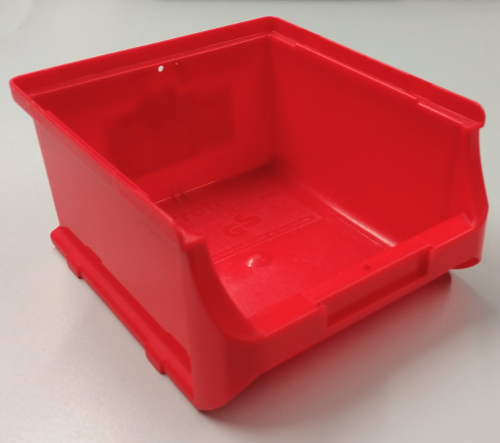
\includegraphics[width=16mm]{images/container_red}}
			\hfill{}
			\subfigure[distance tube]{\label{fig:g}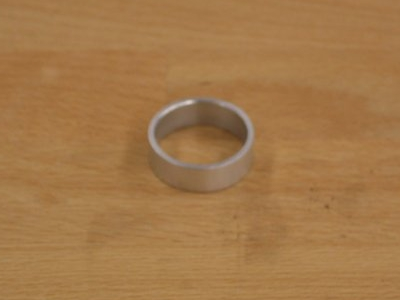
\includegraphics[width=17mm]{images/distanceTube}}
			\hfill{}
			\subfigure[F20\_20\_B]{\label{fig:h}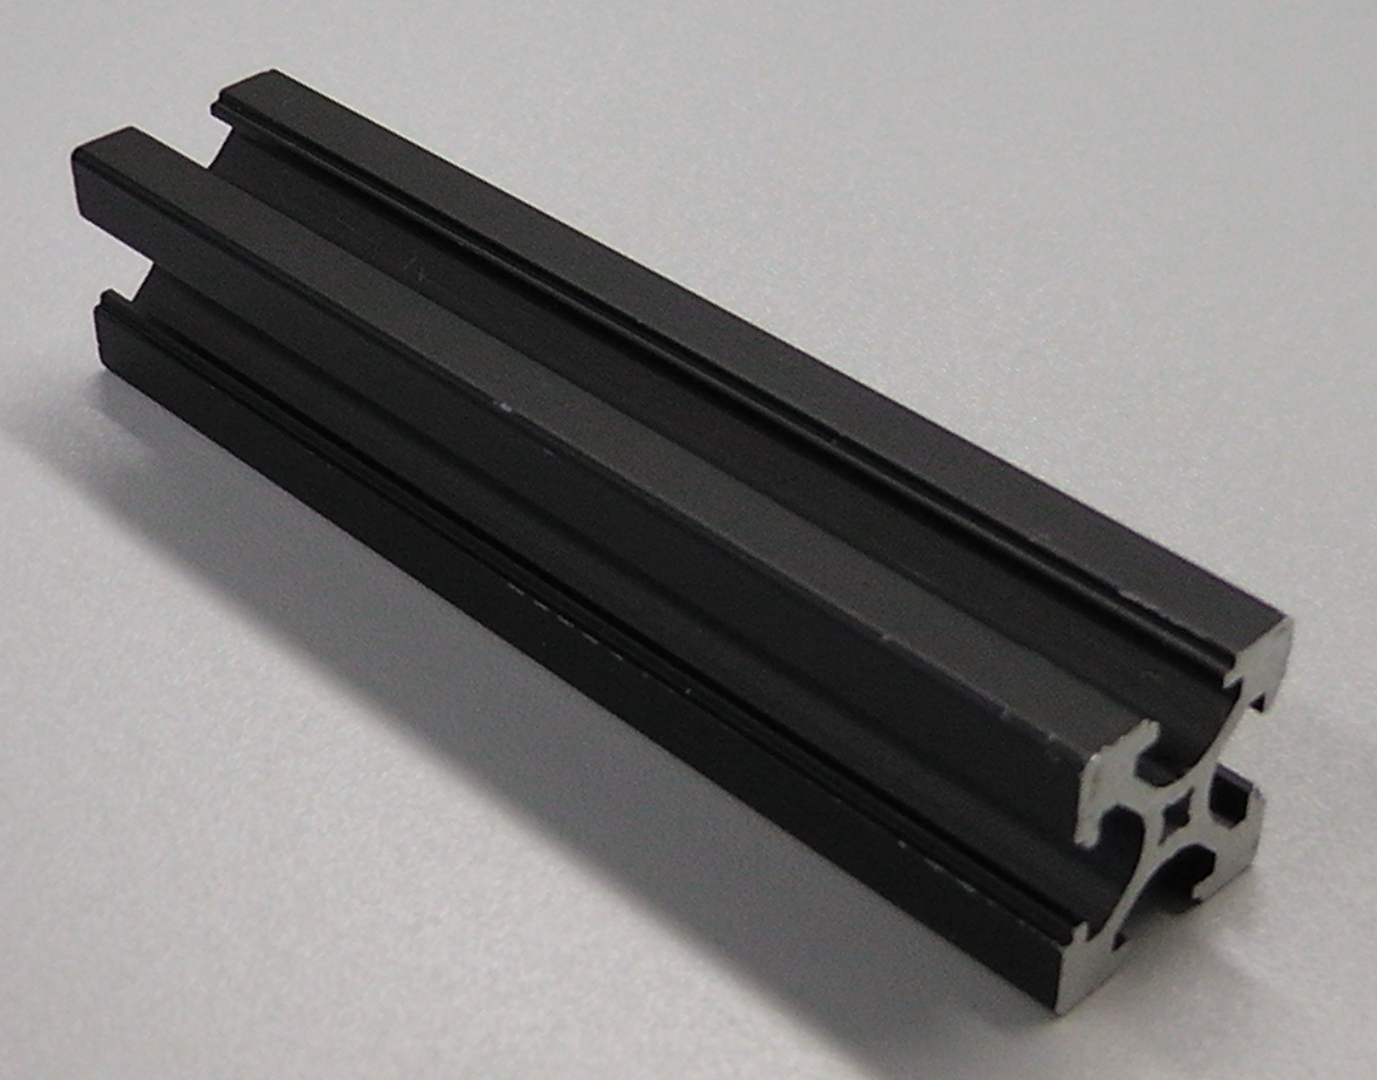
\includegraphics[width=17mm]{images/F20_20_B}}
			\hfill{}
			\subfigure[F20\_20\_G]{\label{fig:i}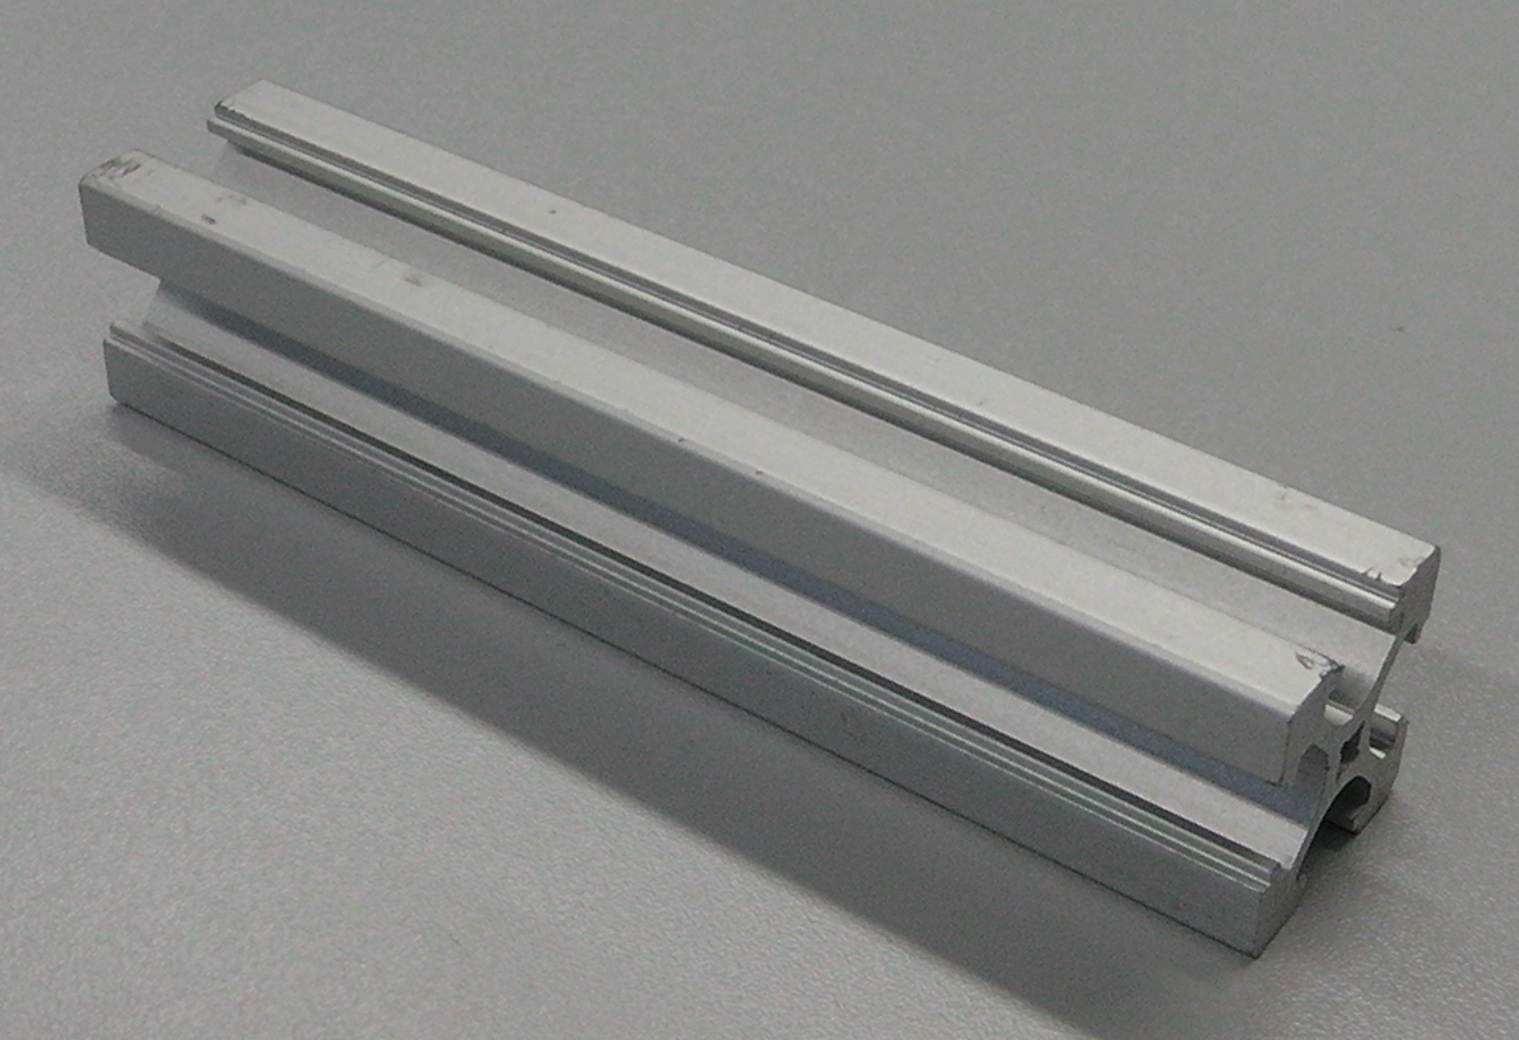
\includegraphics[width=17mm]{images/F20_20_G}}
			\hfill{}
			\subfigure[M20 \cite{github_robocup@work}]{\label{fig:j}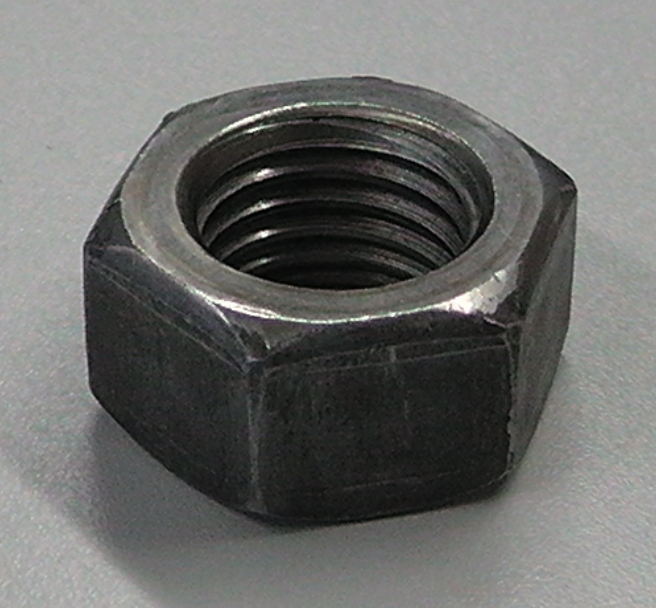
\includegraphics[width=17mm]{images/M20}}
			\hfill{}
			\subfigure[M20\_100]{\label{fig:k}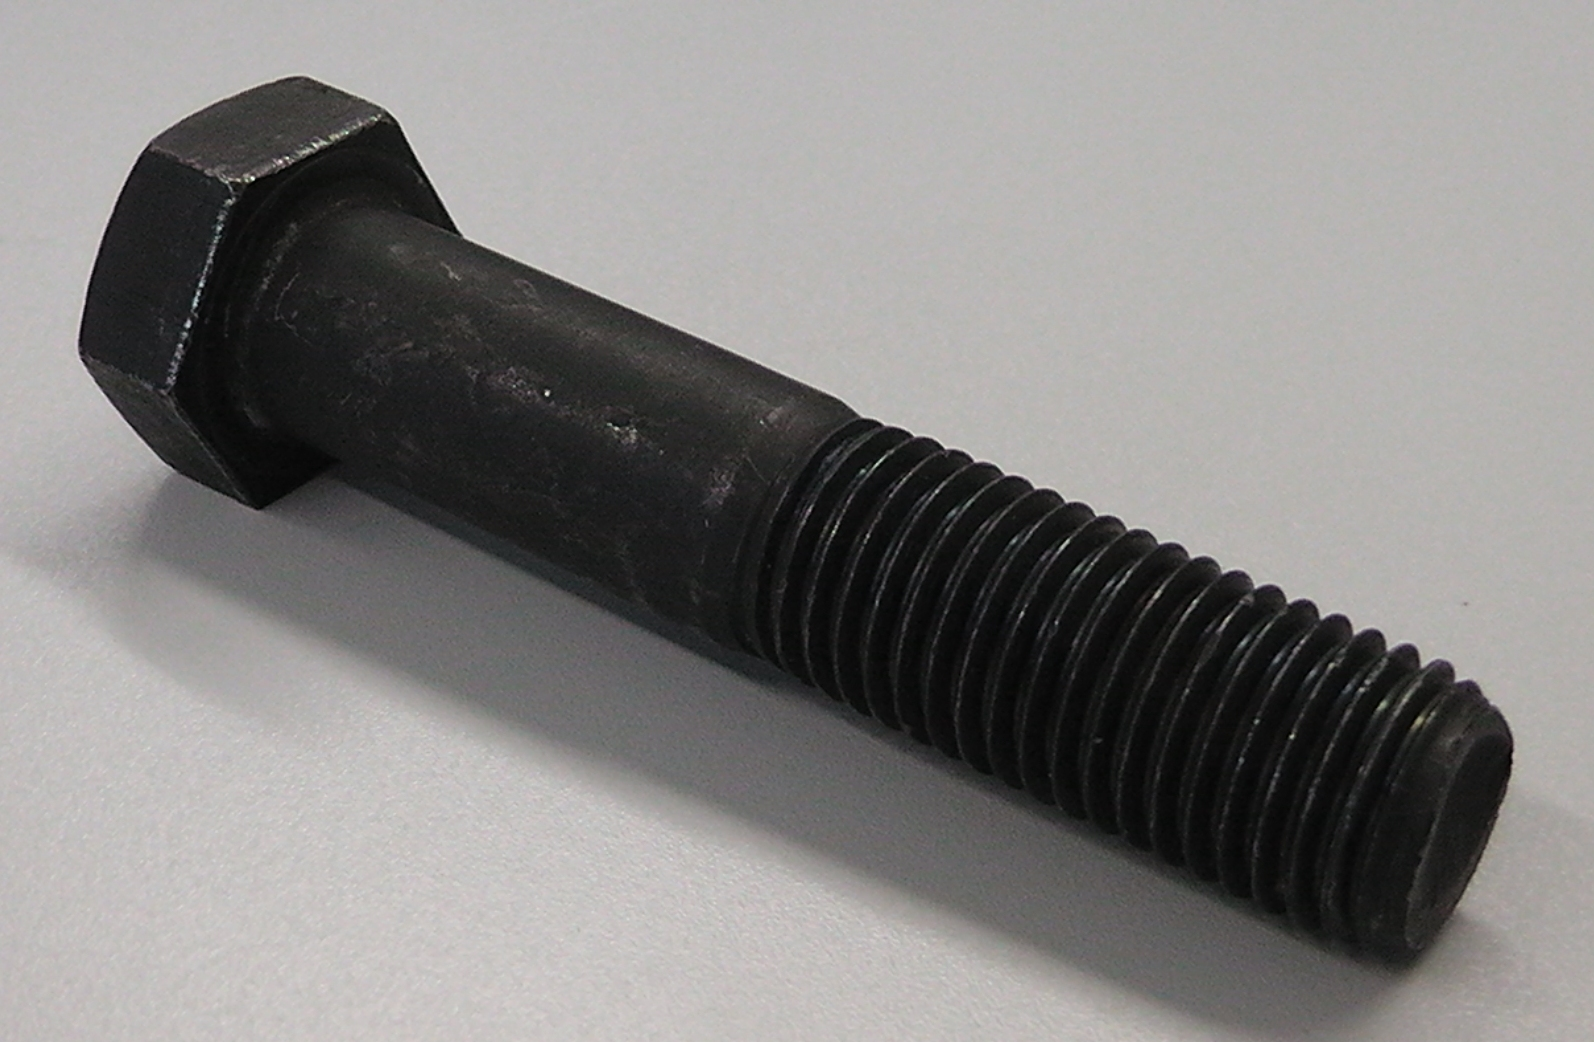
\includegraphics[width=17mm]{images/M20_100}}
			\hfill{}
			\subfigure[M30]{\label{fig:l}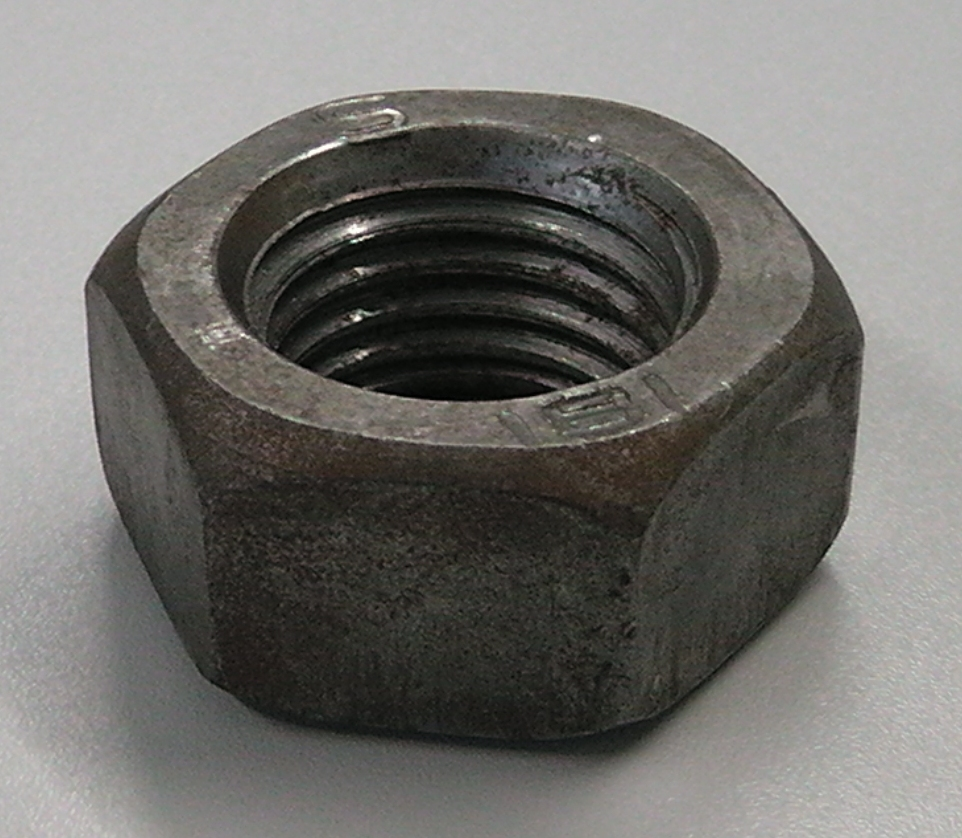
\includegraphics[width=17mm]{images/M30}}
			\caption{Objects in the dataset \cite{github_robocup@work}}
		\end{figure}

\end{frame}

\begin{frame}
	\frametitle{Overview of the dataset}
		\textbf{Objects in the dataset:}
		\begin{figure}
			\centering
			\subfigure[motor]{\label{fig:m}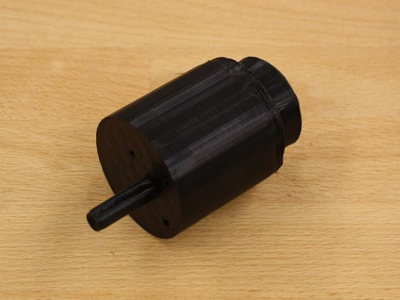
\includegraphics[width=17mm]{images/motor}}
			\hfill{}
			\subfigure[R20]{\label{fig:n}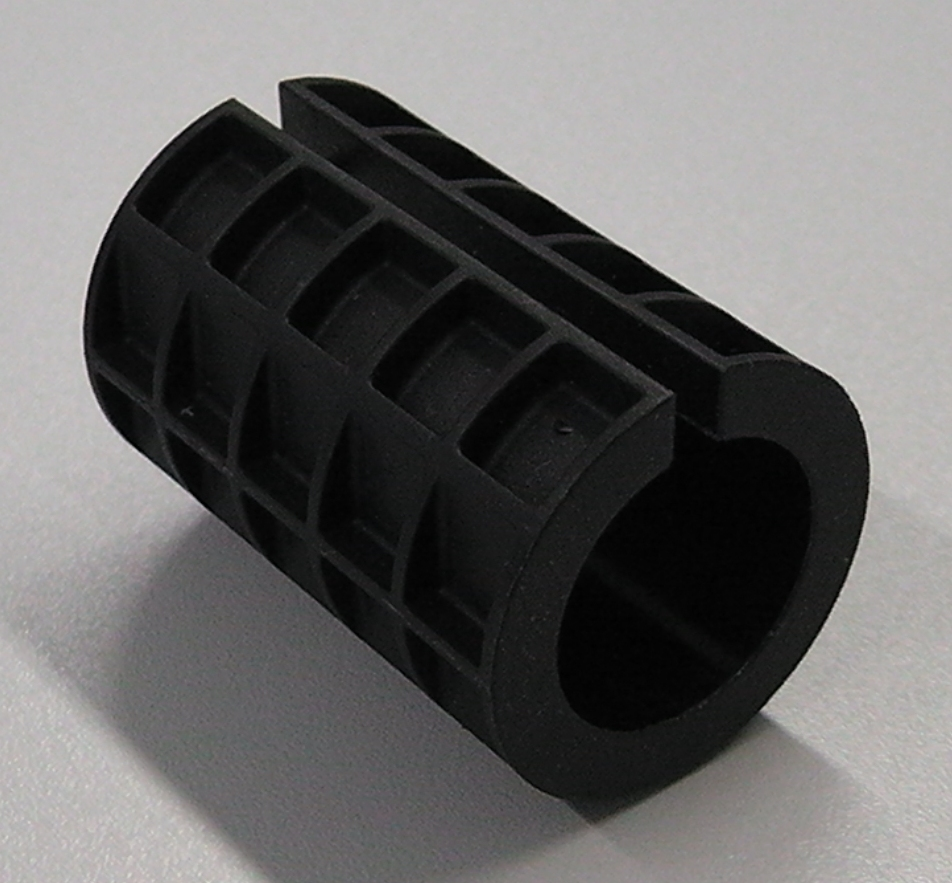
\includegraphics[width=17mm]{images/R20}}
			\hfill{}
			\subfigure[S40\_40\_B]{\label{fig:o}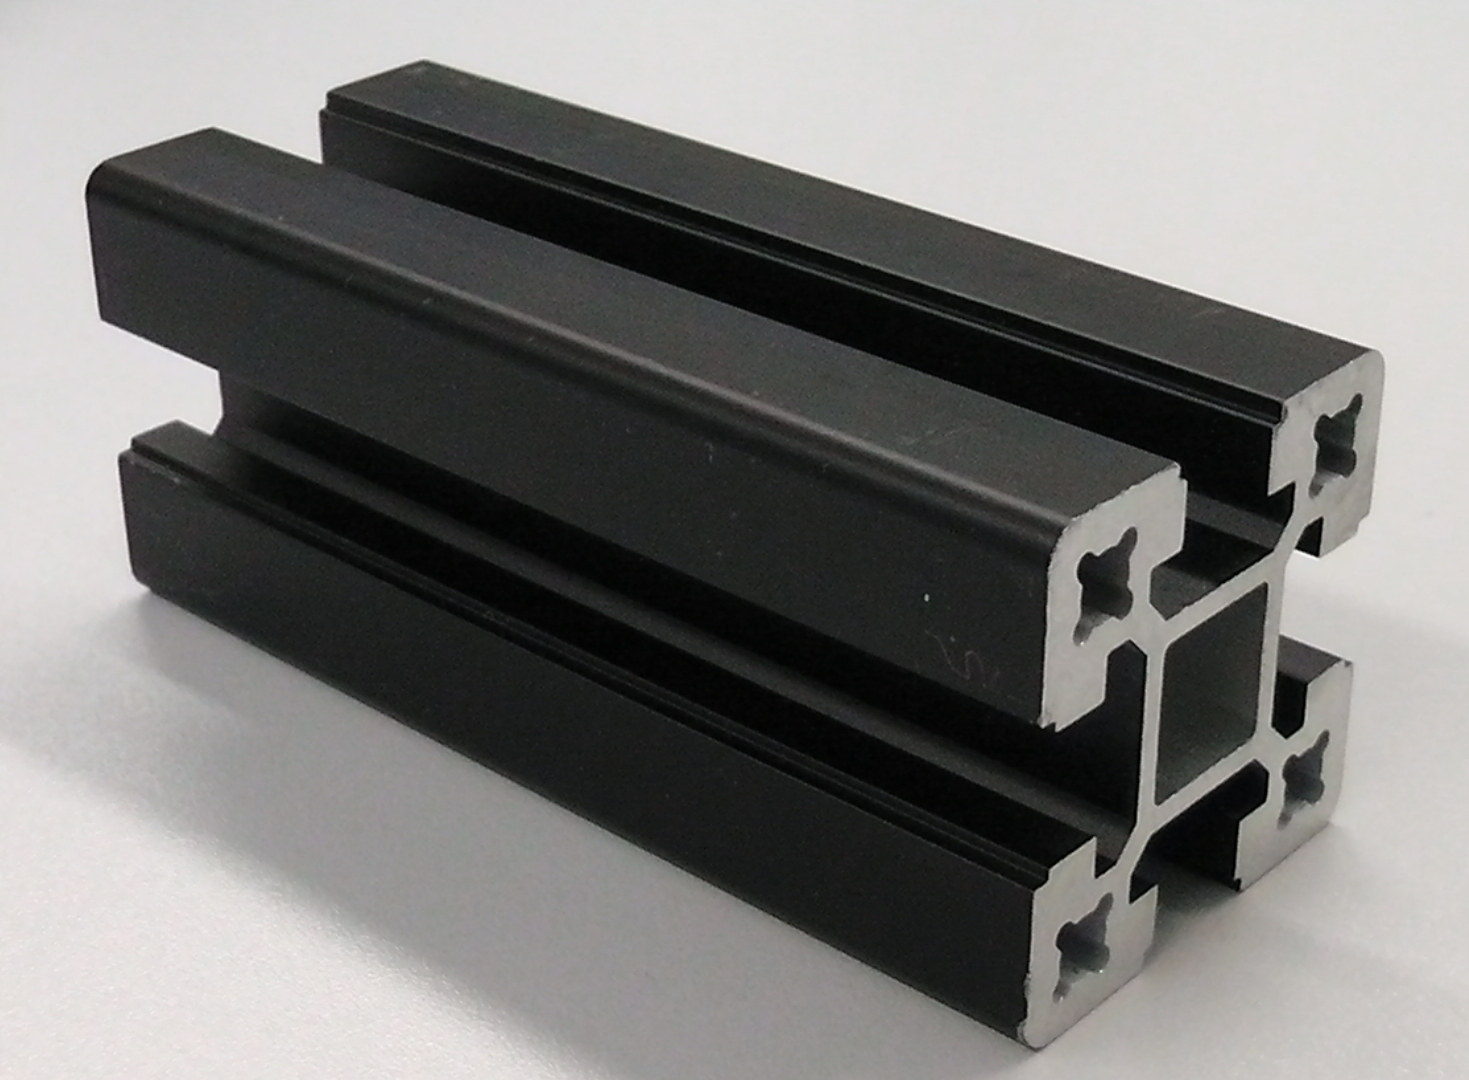
\includegraphics[width=17mm]{images/S40_40_B}}
			\hfill{}
			\subfigure[S40\_40\_G]{\label{fig:p}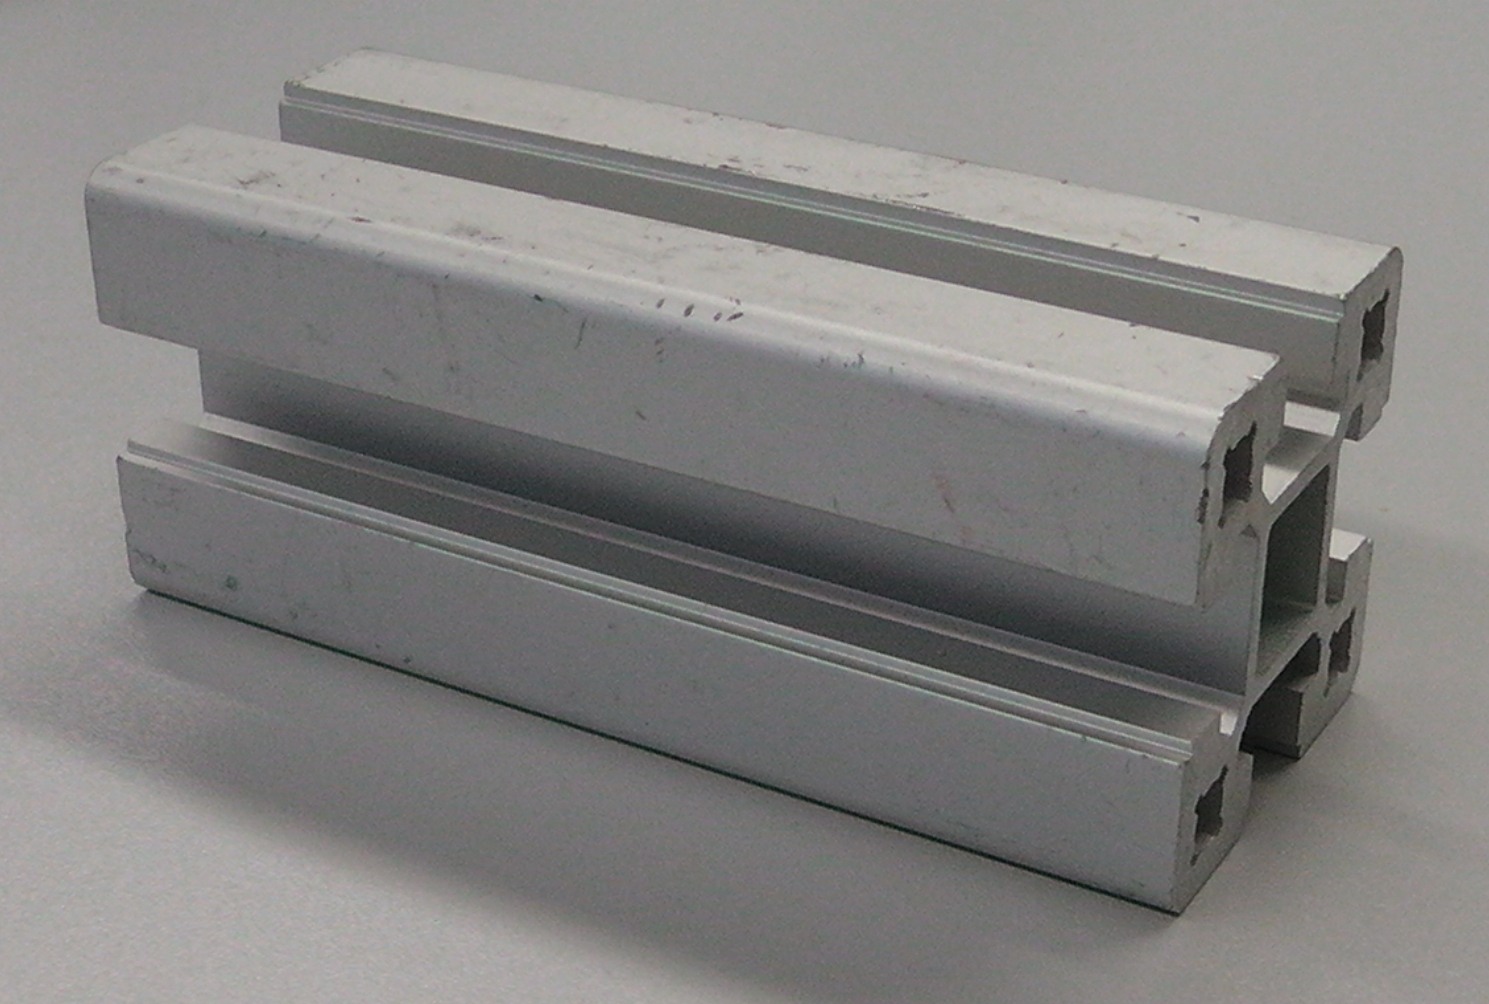
\includegraphics[width=16mm]{images/S40_40_G}}
			\hfill{}
			\subfigure[em\_01]{\label{fig:q}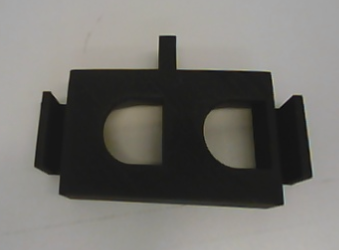
\includegraphics[width=16mm]{images/em_01}}
			\hfill{}
			\subfigure[em\_02]{\label{fig:r}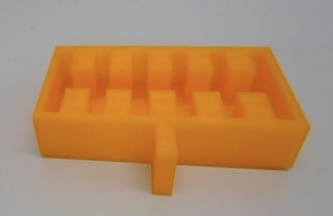
\includegraphics[width=16mm]{images/em_02}}
			\caption{Objects in the dataset \cite{github_robocup@work}}
		\end{figure}

	\begin{itemize}
		\item 18 objects associated to RoboCup @Work are used for the dataset.
		\item 540 images (30 of each object) were taken to create the training dataset.
		\item These images were labeled using the MATLAB ImageLabeler app.
	\end{itemize}

\end{frame}

\begin{frame}
	\frametitle{Motivation behind the augmentation algorithm}
	\section{Motivation behind the augmentation algorithm}
		\begin{itemize}
		\item Manually labeling 540 images using MATLAB ImageLabeler takes roughly 2160 minutes (roughly 4 minutes per image). This is equivalent to around 4 working days. Hence, creating a large dataset with manual labeling is not feasible.
		\item Taking images in a variety of real world backgrounds is also time consuming.
		\item Labeling images with multiple objects would take an even longer time.
	\end{itemize}
	
These drawbacks could be overcome by randomly placing objects on a variety of different background images automatically using an algorithm.
\end{frame}

\begin{frame}
	\frametitle{About the augmentation algorithm}
	\section{About the augmentation algorithm}
		\begin{itemize}
			\item 150 background images were downloaded from the internet using "Google Images Download" \cite{google_images_download} with the keywords: 1. 640x480 background images, 2. 640x480 textured images and 3. 640x480 wallpapers.
			\vspace{3mm}
			\item Using the object locations obtained from manually labeled images, objects were extracted and placed randomly in different locations and scales on these backgrounds.
			\vspace{3mm}
			\item The algorithm provides several tunable parameters which control the occlusions between objects and other aspects as detailed in the dataset report.
			\vspace{3mm}
			\item The algorithm can additionally also provide object detection labels.
		\end{itemize}
\end{frame}

\begin{frame}
	\frametitle{Sample results}
	\section{Sample results}
		\begin{figure}
			\centering
			\subfigure[Sample result 1]{\label{fig:r}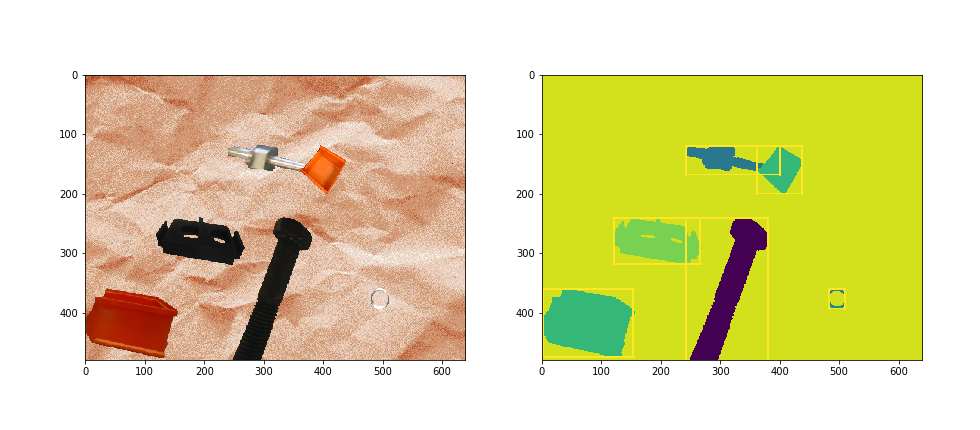
\includegraphics[width=60mm]{images/sample_result_1}}
			\subfigure[Sample result 2]{\label{fig:r}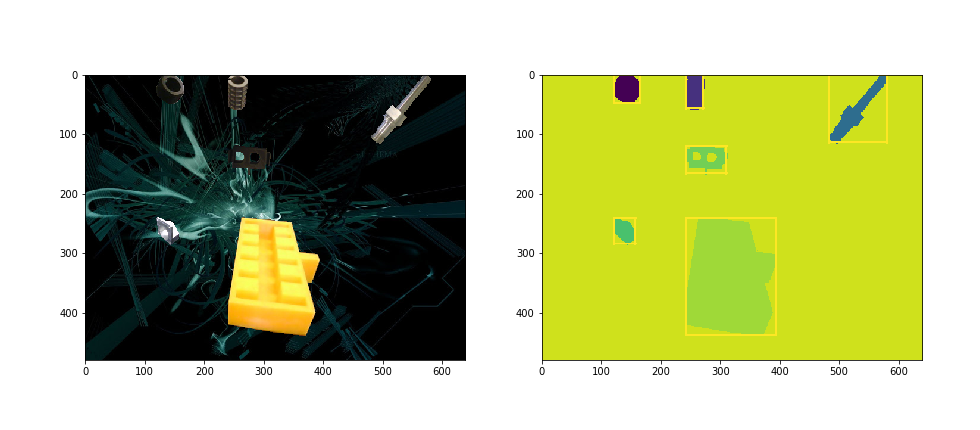
\includegraphics[width=60mm]{images/sample_result_2}}
			\subfigure[Sample result 3]{\label{fig:r}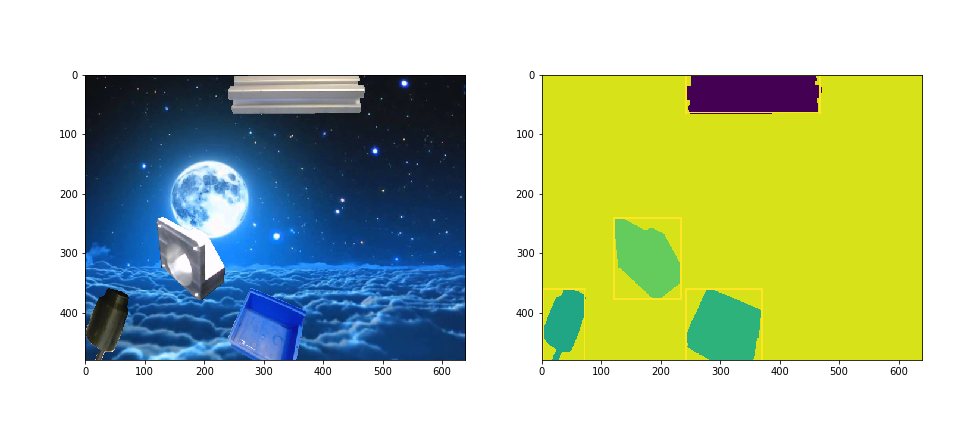
\includegraphics[width=60mm]{images/sample_result_3}}
			\subfigure[Sample result 4]{\label{fig:r}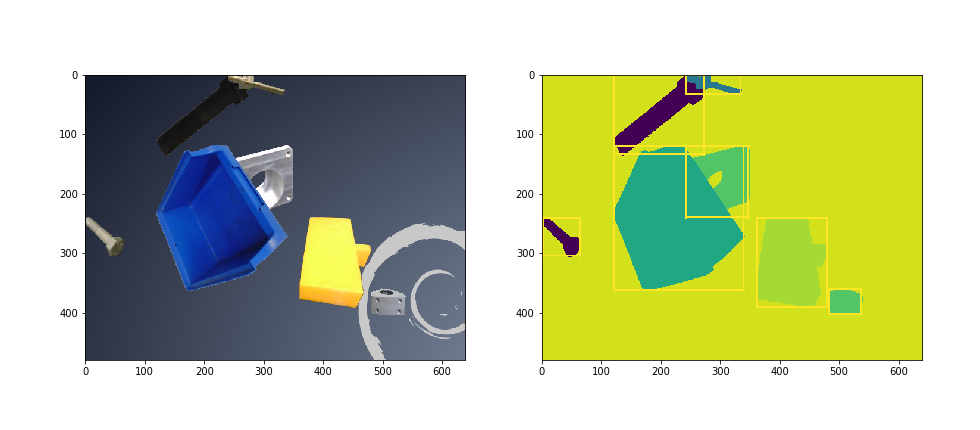
\includegraphics[width=60mm]{images/sample_result_4}}
			\caption{Sample results}
		\end{figure}

\end{frame}

\begin{frame}
	\frametitle{Meta-data of the dataset}
	\section{Meta-data of the dataset}
		Details regarding the dataset is provided in table \ref{Table:1}.

		\begin{table}[!htb]
		\centering
			\begin{tabular}{|c|c|c|c|c|c|c|c|}
			\hline 
    				& Training & Validation & Test \\ 
			\hline 
				\makecell{Real \\Images} & \makecell{30 per object.\\ Total: 30$\times$18=540} & \makecell{5 per object.\\ Total: 5$\times$18=90} & \makecell{5 per object.\\ Total: 5$\times$18=90} \\ 
			\hline 
				\makecell{Augmented\\ Images} & 5000 & 810 & 810 \\ 
			\hline 
				\makecell{Total\\ Images} & 5540 & 900 & 900 \\ 
			\hline 
			\end{tabular}
		\caption{Meta-data of the dataset} 
		\label{Table:1}
		\end{table}

\end{frame}

\begin{frame}
	\frametitle{Selected segmentation architectures for training}
	\section{Selected segmentation architectures for training}
		\textbf{Focus on accuracy:}
		\vspace{3mm}
		\begin{itemize}
			\item[1] Deeplab v3+ \cite{deeplabv3plus2018}:
				\begin{itemize}
					\item Currently holds the second position in cityscapes leaderboard \cite{cityscapes_leaderboard}.
					\vspace{2mm}
					\item Implementation is available in the tensorflow/models repository \cite{tf_models_deeplab}.
					\vspace{2mm}
					\item Uses Xception backbone to reduce computation time and memory requirements.
				\end{itemize}
			\vspace{3mm}
			\item[2] PSPNet \cite{DBLP:journals/corr/ZhaoSQWJ16}:
				\begin{itemize}
					\item Currently among the top 10 in the cityscapes leaderboard \cite{cityscapes_leaderboard}.
					\vspace{2mm}
					\item Different sources of implementations are available.
					\vspace{2mm}
					\item The authors attempt to reduce global context information loss between sub-regions of the input image which is essential for semantic segmentation.
				\end{itemize}
		\end{itemize}
\end{frame}

\begin{frame}
	\frametitle{Selected segmentation architectures for training}
		\textbf{Focus on resource consumption:}
		\vspace{3mm}
		\begin{itemize}
			\item[3] ICNet \cite{DBLP:journals/corr/ZhaoQSSJ17}:
				\begin{itemize}
					\item Focus on attaining real time inference by using a cascade of networks without significant loss of accuracy. 
					\vspace{2mm}
					\item Input image is taken in 3 different resolutions. Most of the computations is performed on the low resolution image and the computations performed on higher resolution image is only intended to improve prediction of small objects.
					\vspace{2mm}
				\end{itemize}
			\vspace{3mm}
			\item[4] MobileNet v2 \cite{mobilenetv22018}:
				\begin{itemize}
					\item Focus on memory efficient inference by using depthwise separable convolutions and other techniques.
					\vspace{2mm}
					\item The authors also evaluate the use of mobileNet v2 on semantic segmentation (in addition to image classification).
					\vspace{2mm}
					\item Implementation is available in the tensorflow/models repository \cite{tf_models_mobilenetv2}.
				\end{itemize}
		\end{itemize}
\end{frame}

\begin{frame}
	\frametitle{Pending tasks}
	\section{Pending tasks}
		\begin{itemize}
			\item Training the 4 selected segmentation models on the created dataset and reporting results.
			\item Finalizing pruning and quantization methods.
			\item Finding and using implementations of the finalized pruning and quantization methods.
			\item Reporting the effects of pruning and quantization on the 4 selected segmentation models.
		\end{itemize}
\end{frame}

\begin{frame}
	\frametitle{References}
	\section{References}
	\printbibliography[title={References}]   
\end{frame}

\end{document}
